\subsection{Description of MSRE Pump Transient Tests}

The \gls{MSRE} was an experimental molten salt reactor constructed and operated at \gls{ORNL} in
the 1960s \cite{haubenreich_experience_1970}. It is a 8-MW$_{\text{th}}$, thermal-spectrum reactor
with a graphite moderator and a LiF-BeF$_2$-ZrF$_4$-UF$_4$ fuel-molten salt mixture. Under normal
power operation, the fuel salt flows out of the core and deposits heat in the heat exchanger before
being pumped back into the core. Due to
\glspl{DNP} being produced in the molten salt coolant, flow rates have significant impacts on the
\gls{DNP} distribution and reactivity. Delayed neutrons born in regions of lower neutronic
importance, e.g., at the periphery or outside the core, are more likely to be lost through neutron
leakage or parasitic absorption.

\gls{ORNL} researchers performed fuel pump start-up and coast-down transient experiments to
determine the ``transient effects of fuel flow-rate changes on reactivity''
\cite{prince_zero-power_1968}. These experiments were a part of \gls{MSRE} zero-power dynamics
tests performed in June 1965, the same month the \gls{MSRE} achieved initial criticality. Figures
\ref{fig:msre-startup} and \ref{fig:msre-coastdown} show the pump speeds and secondary salt coolant
flow rates measured during the transients. The changing flow rates caused advective changes to the
\gls{DNP} distribution and the \gls{DNF} in the reactor core.

During both experiments, the reactivity effects of the \gls{DNP} drift were measured by
allowing the flux servo controller to maintain criticality. The controller maintained core
criticality by adjusting the control rod insertion height in response to \gls{DNP} drift-induced
reactivity changes. The reactivity changes over time can be calculated by comparing the various
control rod positions (Figure \ref{fig:msre-pump-rod}) with the control rod integral worth curve
(Figure \ref{fig:msre-rod-worth}) obtained during control rod calibration experiments.

\begin{figure}[htb]
  \centering
  \begin{minipage}[t]{0.49\textwidth}
    \centering
    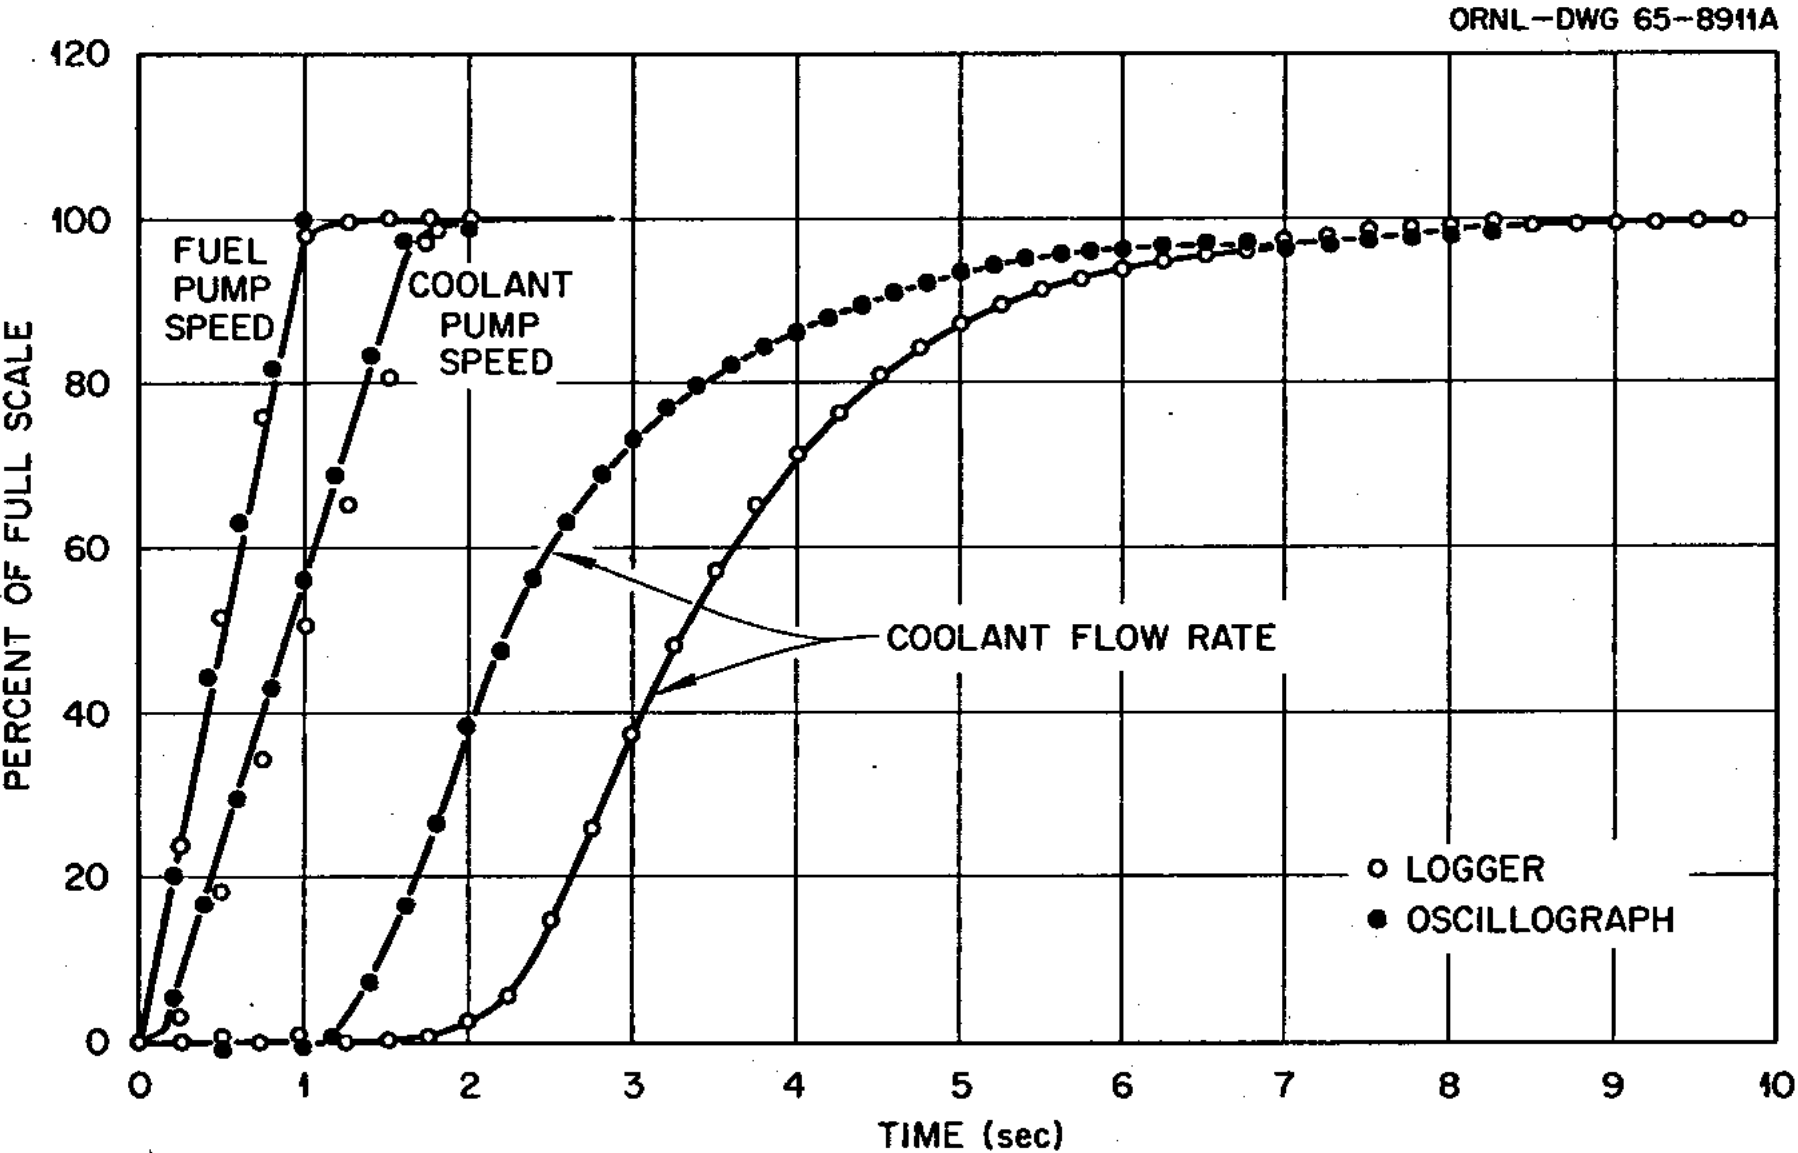
\includegraphics[width=\columnwidth]{msre-startup}
    \caption{Start-up pump speed and coolant flow rate \cite{prince_zero-power_1968}.}
    \label{fig:msre-startup}
  \end{minipage}
  \hfill
  \begin{minipage}[t]{0.49\textwidth}
    \centering
    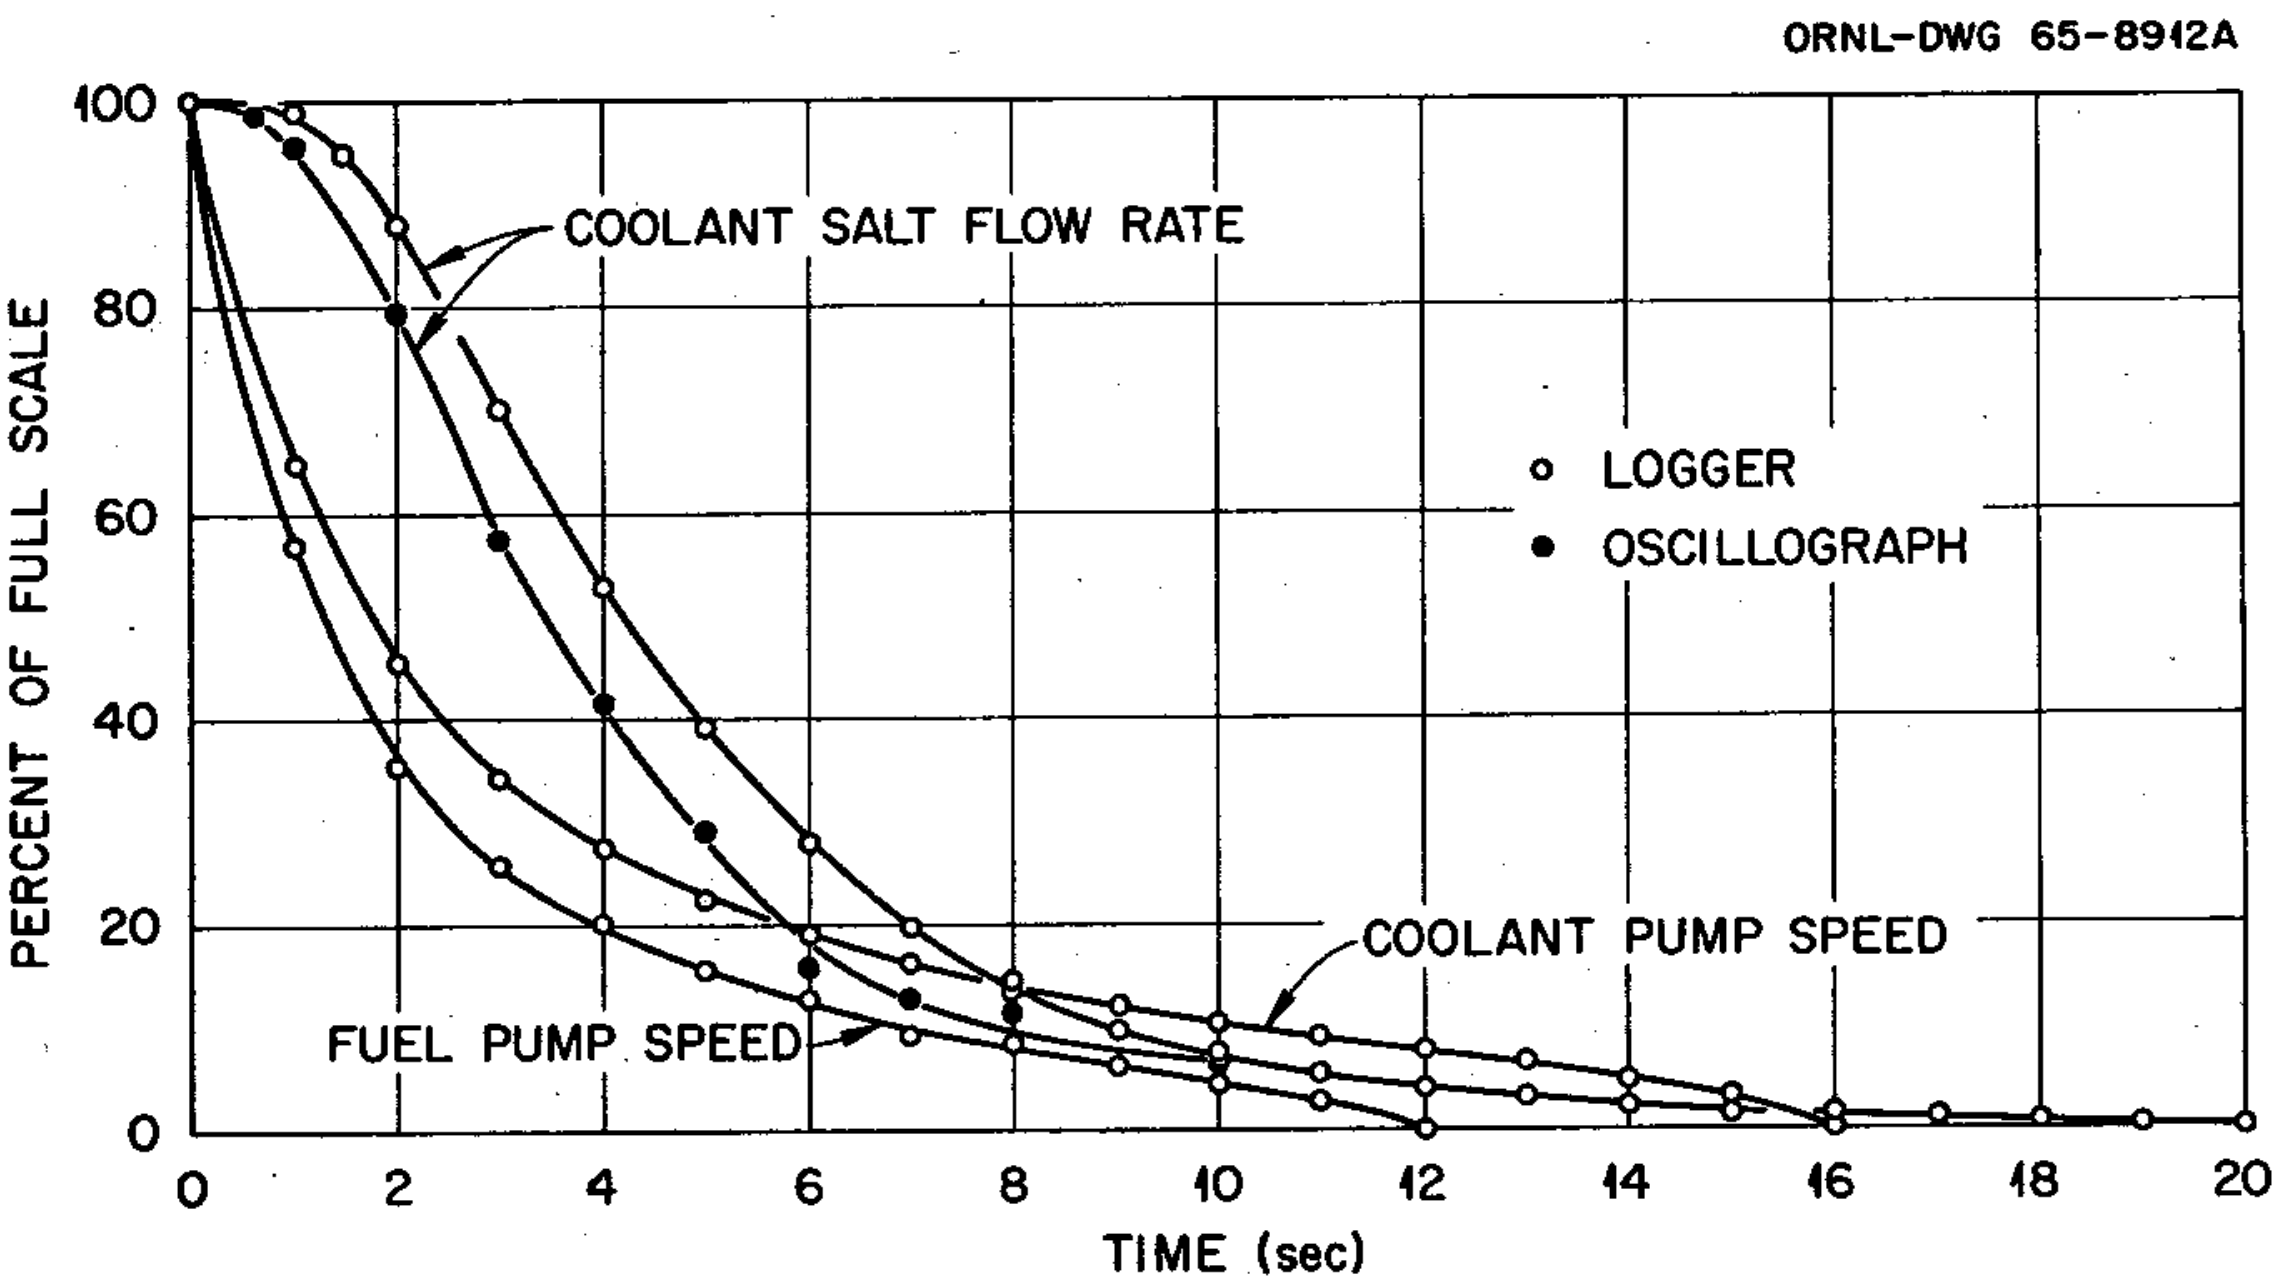
\includegraphics[width=\columnwidth]{msre-coastdown}
    \caption{Coast-down pump speed and coolant flow rate \cite{prince_zero-power_1968}.}
    \label{fig:msre-coastdown}
  \end{minipage}
\end{figure}

\begin{figure}[htb]
  \centering
  \begin{minipage}[t]{0.49\textwidth}
    \centering
    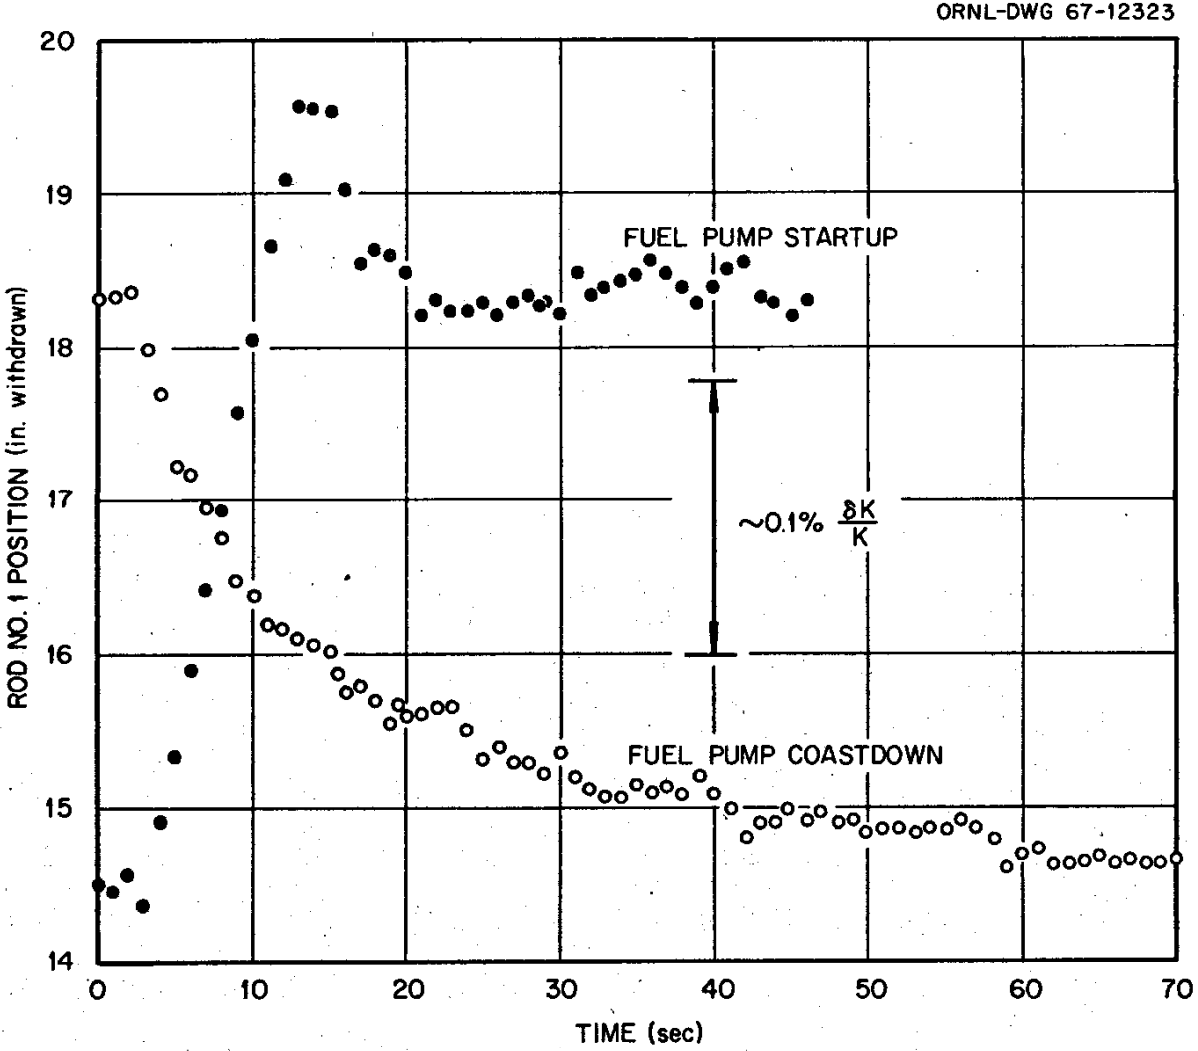
\includegraphics[width=\columnwidth]{msre-transient}
    \caption{Control rod response to fuel pump start-up and coast-down
    \cite{prince_zero-power_1968}.}
    \label{fig:msre-pump-rod}
  \end{minipage}
  \hfill
  \begin{minipage}[t]{0.49\textwidth}
    \centering
    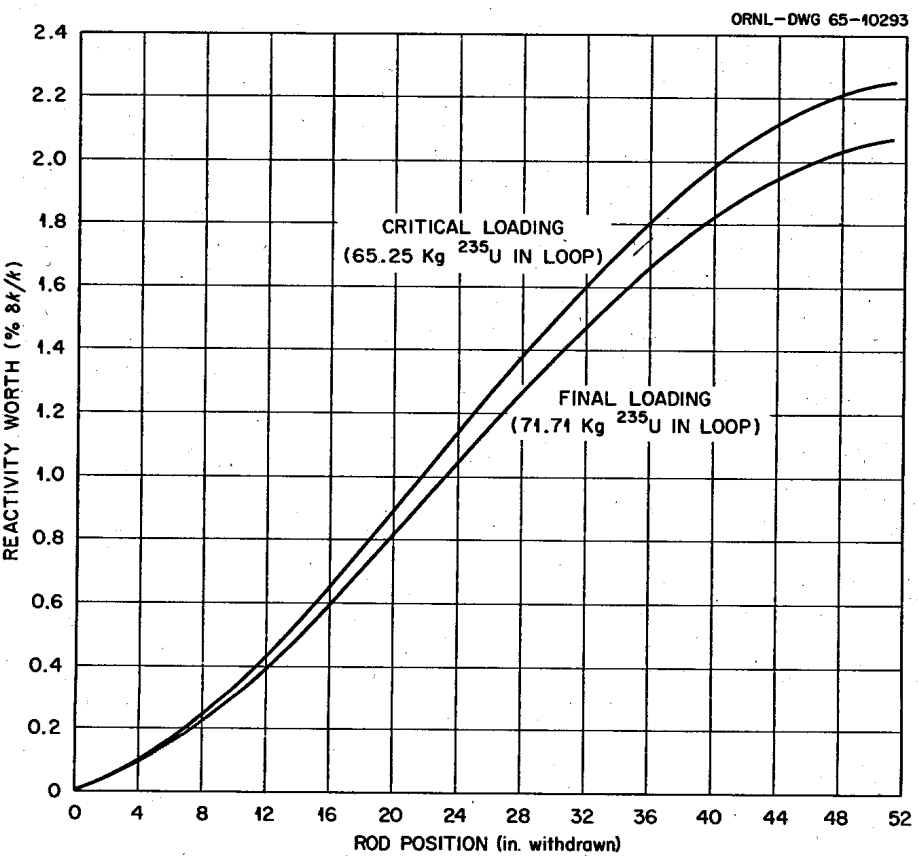
\includegraphics[width=\columnwidth]{msre-rod-worth}
    \caption{Integral control rod worth of Rod 1 \cite{prince_zero-power_1968}.}
    \label{fig:msre-rod-worth}
  \end{minipage}
\end{figure}


\subsection{Modeling Approach}

\subsection{Results}

\subsection{Summary}

\FloatBarrier
